\documentclass[12pt,a4paper]{article}
\usepackage[utf8x]{inputenc}
\usepackage{ucs}
\usepackage{amsmath}
\usepackage{amsfonts}
\usepackage{amssymb}
\usepackage{graphicx}
\usepackage{listings}
\usepackage[left=2cm,right=2cm,top=2cm,bottom=2cm]{geometry}

\usepackage{natbib}
\bibpunct{[}{]}{,}{n}{}{;}

\usepackage[pdftex,pagebackref]{hyperref}
    \usepackage{natbib}
    \hypersetup{colorlinks,linktocpage=true}
\renewcommand{\backrefpagesname}{ \protect\\  \textit{Cited on
page(s):}~}
\renewcommand{\backref}{\backrefpagesname}

\author{Gergely Imreh}
\title{Quadruple coil drive circuits}
\date{2013-03-22, v1}
\begin{document}
\maketitle

\tableofcontents

\section{Requirements}

The coils in the experimental system creating the quadruple magnetic field have much higher requirements than the usual MOT experiments. Have to create very large magnetic field gradients, and have to ramp, switch on/off in a short time.

The stated requirements for the circuit to performa are: 
\begin{itemize} \itemsep -2pt
\item Being able to supply up to 400A (because of the required magnetic field)
\item Switching on in $\sim$millisecond, and off in few hundred microsecond (explicit requirement)
\item Ramping between the 100\% and ~20\% in a few seconds (from similar experiment's paper)
\end{itemize}


\section{Semiconductor selection}

There are quite a few different sources about MOSFET and IGBT differences and choosing between them, for some more information than explicitely shown here, can see \citet{Blake,Linder2006,Melito2005}.

There is not too much difference between the two, because the actual technology is so very similar, see Fig. \ref{fig:comparison1} for their comparative cross section. Most of the differences between BJT, MOSFET and IGBT are summarized in Table \ref{tab:semicompare}.

\begin{figure}[ht!]
\centering
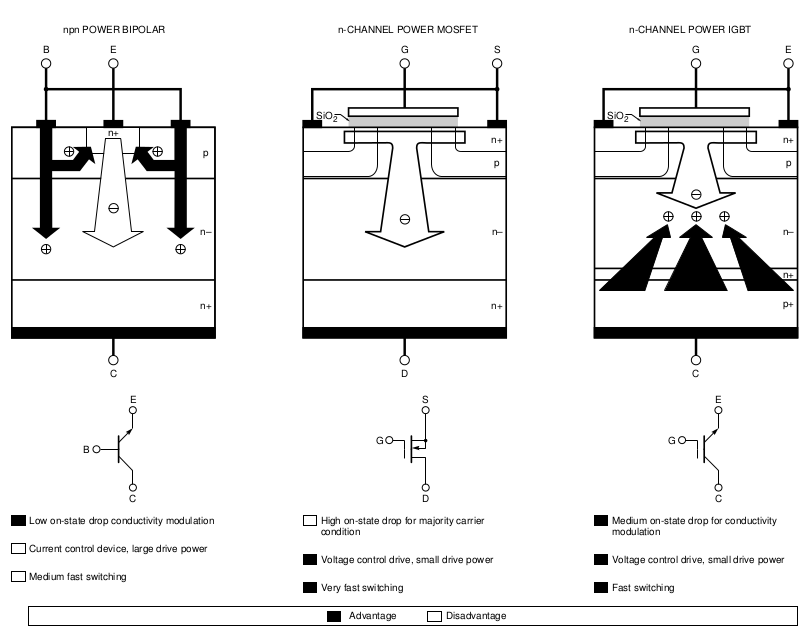
\includegraphics[width=150mm]{comparison1.png}
\caption{Comparison of BJT, MOSFET, and IGBT, from \citep{Blake}{MitsubishiIGBT}.}
\label{fig:comparison1}
\end{figure}

\begin{table}[ht!]
\centering
\begin{tabular}{|c|c|c|}
\hline 
BJT & MOSFET & IGBT \\ 
\hline 
Current controlled & Voltage controlled & Voltage controlled \\ 
\hline 
Slow turn off & Quick turn off & Medium turn off \\ 
\hline 
High power & Medium power & High power \\ 
\hline 
Low frequency operation & High frequency operation & Low frequency operation \\ 
\hline 
Thermal runaway & No thermal runaway & Thermal runaway \\ 
\hline 
Moderate on-state voltage drop & Low on-state voltage drop & Low on-state voltage drop \\ 
\hline 
Does not latch up & Does not latch up & Older versions latched up \\ 
\hline 
\end{tabular} 
\caption{Comparison of available power semiconductor technologies, based on \citet{Gorelik2002}}
\label{tab:semicompare}
\end{table}

\subsection{MOSFET}

So far, the main things to consider about MOSFETs are the following. Usually they have lower current threshold than IGBTs, and they are designed for lower voltage operation. If the current threshold is too low for the application, can use a number of them in parallel, but one has to be careful with the switch timing, there can be differences between the delay times of the different pieces of MOSFET, thus it might require sychnronization. Their thermal behaviour might be better since there's no thermal runaway, and might be easier to handle their cooling because of that.

There's one standard characterization (and thus a standard work setting) of MOSFETS which is very similar to the planned circuit, called Unclamped Inductive Switching (UIS). It's basically switching off an inductive load. During the switch-off time, the total energy discipated in the MOSFET is \cite{Linder2006}:
\begin{equation}
E_{\mathrm{avalanche}} = L_{\mathrm{load}} \frac{I_L^2}{2} \frac{V_{\mathrm{max}}}{V_{\mathrm{max}}-V_{\mathrm{DC}}}
\end{equation}
where $V_{\mathrm{max}}$ is the maximum voltage across the transistor (e.g. breakdown voltage), and $V_{\mathrm{DC}}$ is the supply voltage. The specs should say the maximum of this $E_{\mathrm{avalanche}}$ for the given MOSFET. In practice, this might not matter here, because in this circuit, the voltage should be clamped. The switching time still depends on the maximum voltage the component can take, thus in general I think even if MOSFET can switch faster, the circuit behaviour will be dominated by the slower inductive current decay.

\subsection{IGBT}

In general, the behaviour of the IGBTs are very similar to MOSFETs, to that extent, that most of its switching behaviour can be described the same way as those. The main differences seen so far are the following. There's a longer current tail when switching off, because of the recombination of the internal charge carriers. This in practice might not make any difference, because the IGBT is still so much faster (generally around or below $1 \mu \mathrm{s}$ switching time) than the rest of the circuit.

It definitely needs better cooling, and more stable temperature, because of it's thermal runaway, and temperature dependent output characteristics.

In general it IGBTs are higher power devices than MOSFETs, thus it's easier to find high current / high voltage ones, to have only a single component to do the switching. They are more stable and rugged in terms of having stable long-term characteristics.

For switching tasks (in the electronics meaning of repeated on/off cycles quickly), IGBTs are less suitable because of the current tail, and a consequent longer deadtime, while these are just ``long'' compared to MOSFET.

The IGBTs chosen for the task depends on whether it is only switching that needs to be done (with optional current control via the power supply), or it is required to feedback control the current via the IGBT resistance.

For the first task, switching, a lower voltage IGBT generally has better characteristics. The Microsemi APTGT600A60G\footnote{Microsemi product page: \url{http://www.microsemi.com/existing-parts/parts/59800}} that was bought by Lab107 as well, has the output charactheristics shown on Fig. \ref{fig:microsemi}: the $V_{CE}$ collector-emitter voltage is low, and above a certain threshold $V_G$ gate voltage, it is capable of conducting the full planned current range.

\begin{figure}[ht!]
\centering
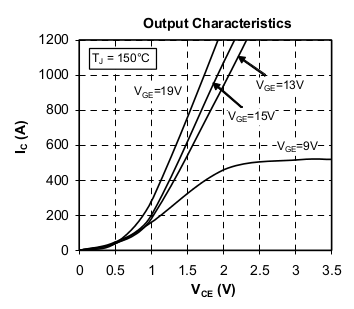
\includegraphics[width=90mm]{Microsemi.png}
\caption{I-V Microsemi APTGT600A60G, product page: \url{http://www.microsemi.com/existing-parts/parts/59800}. It has very low collector-emitter voltage drop, that would be the best for the circuit in constant current operation.}
\label{fig:microsemi}
\end{figure}

For the second taks, feedback controller current, generally higher voltage IGBTs seem to be more suitable, there are more of those that have similar output characteristics as Powerex CM600DY-24S\footnote{Powerex product page \url{http://www.pwrx.com/Product/CM600DY-24S}} has, similar part to the one used in NIST, shown on Fig. \ref{fig:cm600dy}. Here the more important aspect is the low $V_{CE}$ saturation region, thus if one provides $\approx 3V$ voltage drop over the collector-emitter region, the $V_G$ can be used to adjust the current over the entire planned current range (similarly as it is discussed in  \citet{Sattar}).

\begin{figure}[ht!]
\centering
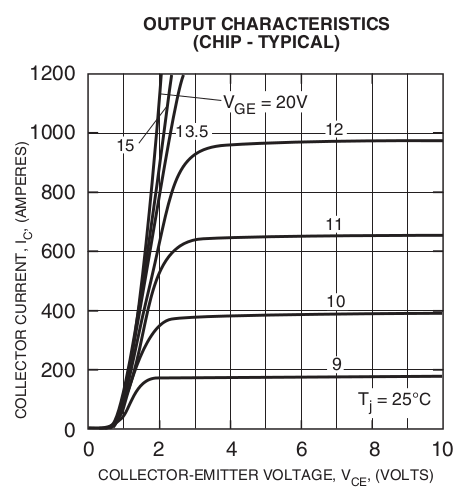
\includegraphics[width=90mm]{CM600DY-24S_I_V.png}
\caption{I-V curve for Powerex (Mitsubishi) CM600DY-24S, product page \url{http://www.pwrx.com/Product/CM600DY-24S}. It has good saturation regions that appear to be useful for current control via the gate voltage.}
\label{fig:cm600dy}
\end{figure}

\section{Complete circuit}

For reference, the (old?) NIST setup is shown on Figure \ref{fig:nistcircuit}. It seems to have a lot in common with most of the other circuits I've seen, except for the varistor, which is here parellel with the coil, while in most cases it is parallel with the IGBT, protecting that from overcurrent. Other than this difference, the arrangement looks like a basic switching circuit. The IGBT used is Powerex CM600HA-24A, which seems now obsolete, but there are straightforward replacements.

\begin{figure}[ht!]
\centering
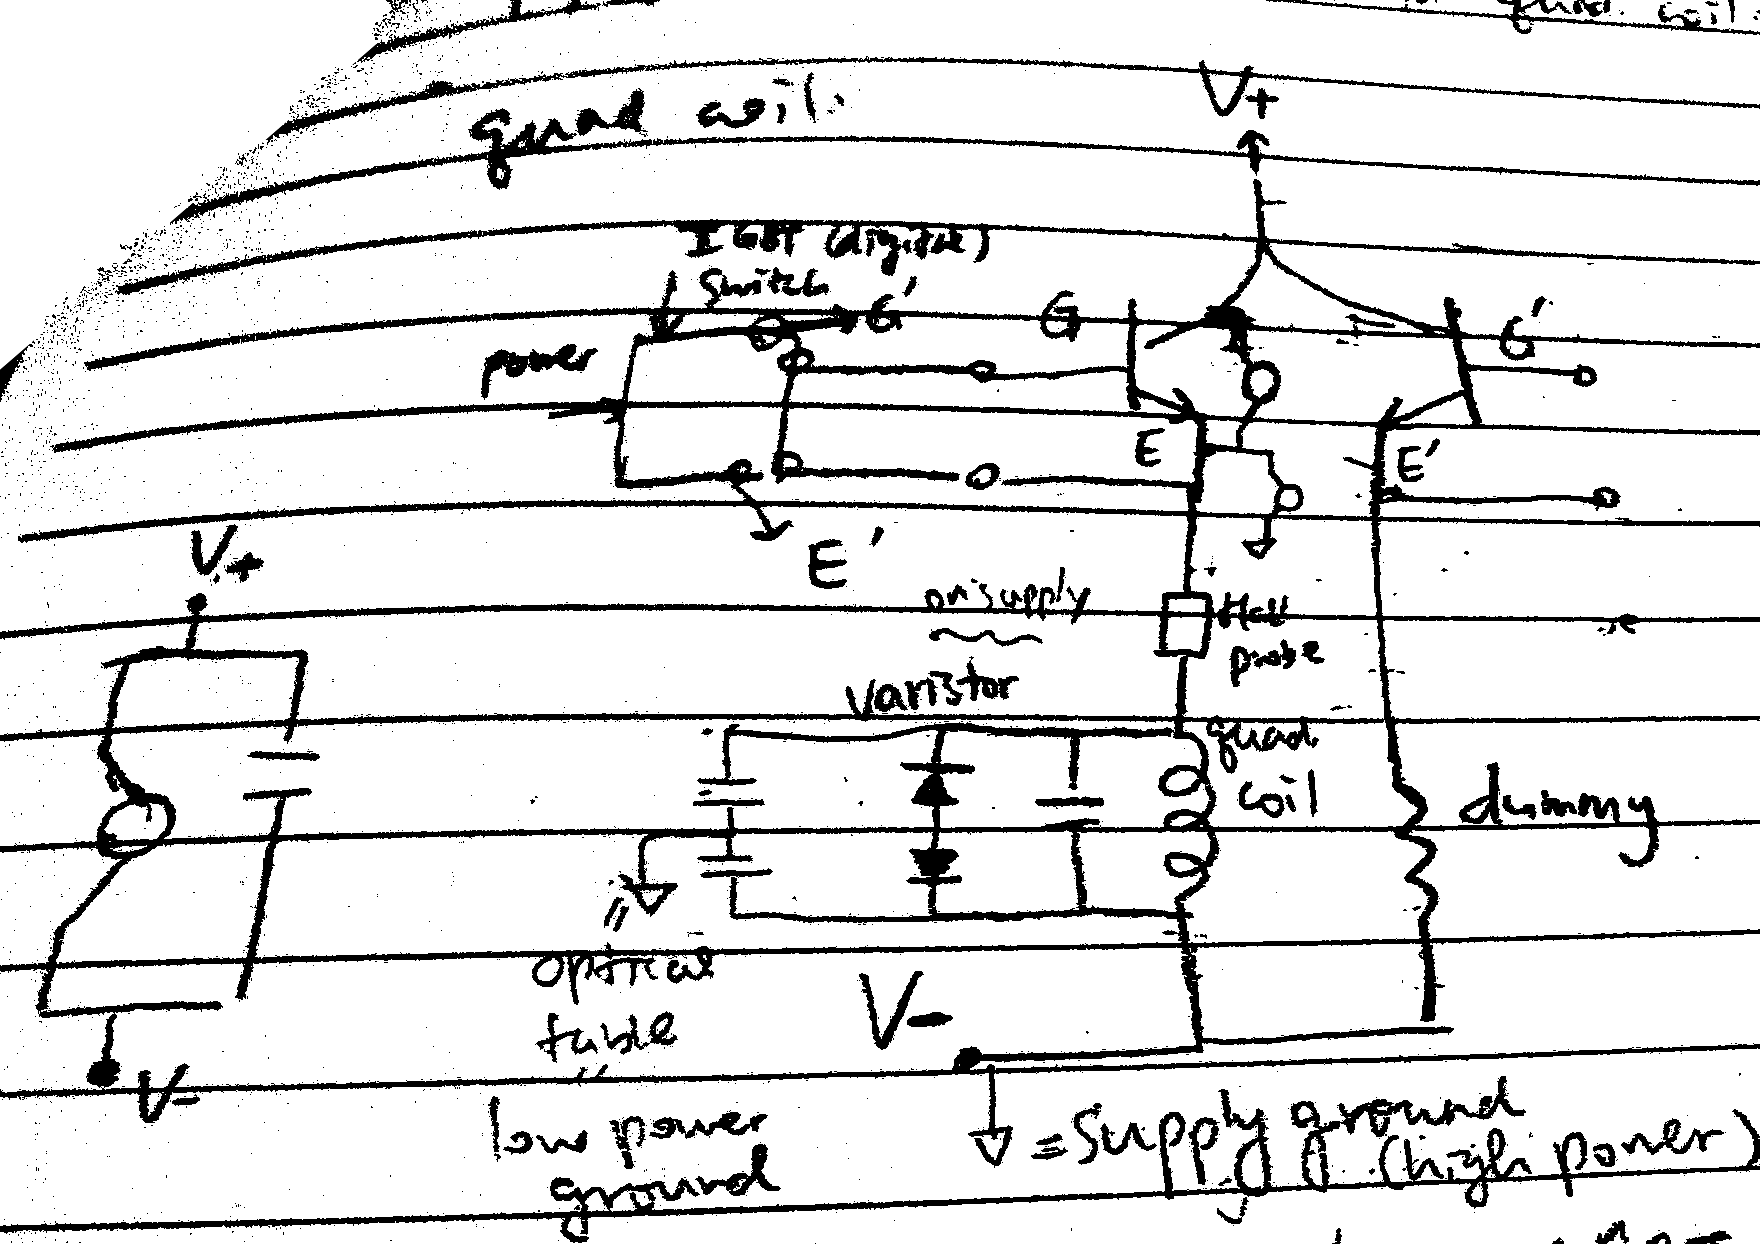
\includegraphics[width=120mm]{NIST.png}
\caption{NIST circuit (2007)}
\label{fig:nistcircuit}
\end{figure}


For the correct prediction of behaviour, the complete circuit has to be taken into account, thus the switching time of the IGBT can be slowed down quite a bit, if the coil's inductive current is not discipated fast enough. For the timing behaviour one can make some estimates using a mathematical model of the circuit using the measured and spec sheet values, similarly as it was done in \citet{Deissler2003}. They also take into account voltage limiting, and as much as I understood, the experimental results are close to their calculation, sub-millisecond switching times with $750A$ switching. Their circuit is shown on Fig \ref{fig:deissler}, they use Powerex CM600HU-12F, all other part numbers are detailed there.

\begin{figure}[ht!]
\centering
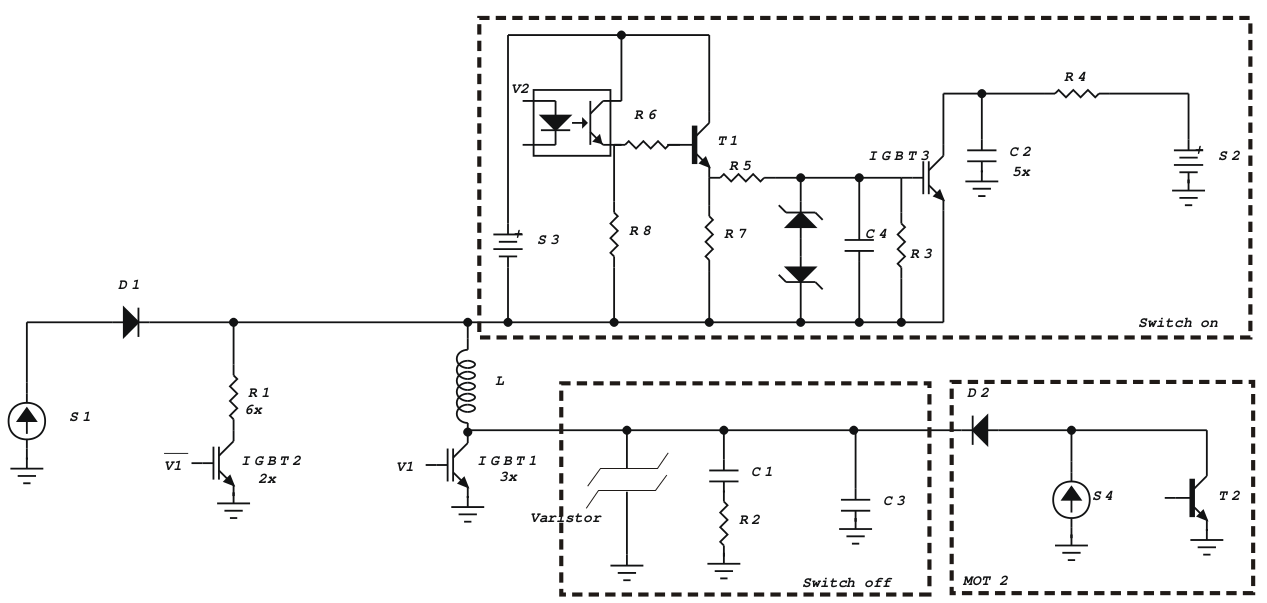
\includegraphics[width=150mm]{Deissler.png}
\caption{Main control circuit from from \cite{Deissler2003}, Fig. 2.1 , component values there in Table 2.1}
\label{fig:deissler}
\end{figure}

Another simple circuit is shown in \citet{Yum2012}, also on Figure \ref{fig:yum2012circuit}. They can use similarly high current, $\approx 400V$, the switching time is not clear, but they do ramping in $10\mathrm{ms}$. The part numbers I got from personal communication\footnote{Dahyun Yum starydh@gmail.com} are: IGBT is Powerex PM800HSA120\footnote{PM800HSA120 product page: \url{http://www.pwrx.com/Product/PM800HSA120}}, varistor TNR20E391K\footnote{TNR20E391K simple specs: \url{http://www.pucko-elektronik.com/download/nwar/tnre.pdf}} ($\times 5$ parallel), diode MDF25A40\footnote{MDF25A40 product page: \url{http://www.galco.com/buy/Sanrex-Sansha-Electric-Manufacturing/MDF250A40}}, resistor Alcol NHS250 1 Ohm ($\times 3$ parallel). The ramping they are likely to do with their power supply (Lambda EMI\footnote{Lambda EMI power supplies: \url{http://www.us.tdk-lambda.com/hp/}}) directly.

\begin{figure}[ht!]
\centering
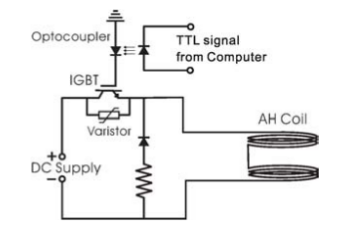
\includegraphics[width=100mm]{Yum2012_circuit.png}
\caption{Simpler current switching from \citet{Yum2012}, part numbers in text. The resistor and varistor are actually $\times 3$ and $\times 5$ parallel connected devices, simplified on the diagram}
\label{fig:yum2012circuit}
\end{figure}

Figure \ref{fig:atomchipcircuit} shows the circuit used in \citet{Aubin2005}. Their performance is 60A off in $150 \mu \mathrm{s}$, 26.5A on in $350 \mu \mathrm{s}$. Difference is their use of Transient Voltage Supressors instead of varistors (though I expect they work rather similarly), and pre-charged capacitors to speed up the switching process (showing up in some other papers as well). Still, due to their lower current, this might not work the same way for the required high current operation.

\begin{figure}[ht!]
\centering
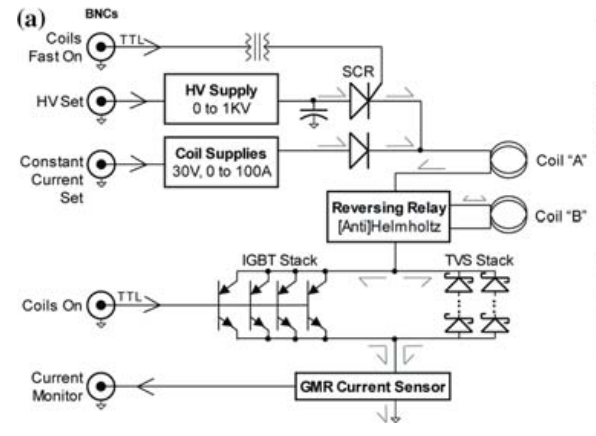
\includegraphics[width=120mm]{atomchipcircuit.png}
\caption{Circuit from from \citet{Aubin2005}.}
\label{fig:atomchipcircuit}
\end{figure}

In \citet{Palittapongarnpim2012} the author use both static current with rapid on/off, Figure \ref{fig:pstaticcircuit}, and current ramp circuit, Figure \ref{fig:pfeedbackcircuit}. It's using lower maximum current, $\approx/ 200 \mu \mathrm{s}$. The feedback control is relatively simple, and I guess there are no real protection circuits because of the lower maximum current.

\begin{figure}[ht!]
\centering
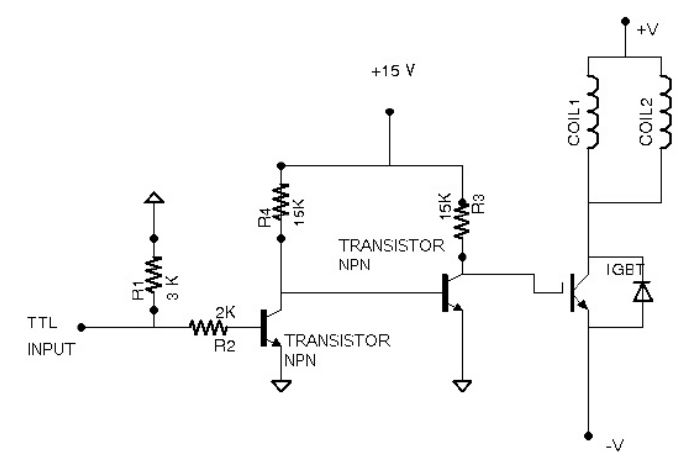
\includegraphics[width=100mm]{static_circuit.png}
\caption{Static current control circuit from \cite{Palittapongarnpim2012}, Fig 3.9}
\label{fig:pstaticcircuit}
\end{figure}

\begin{figure}[ht!]
\centering
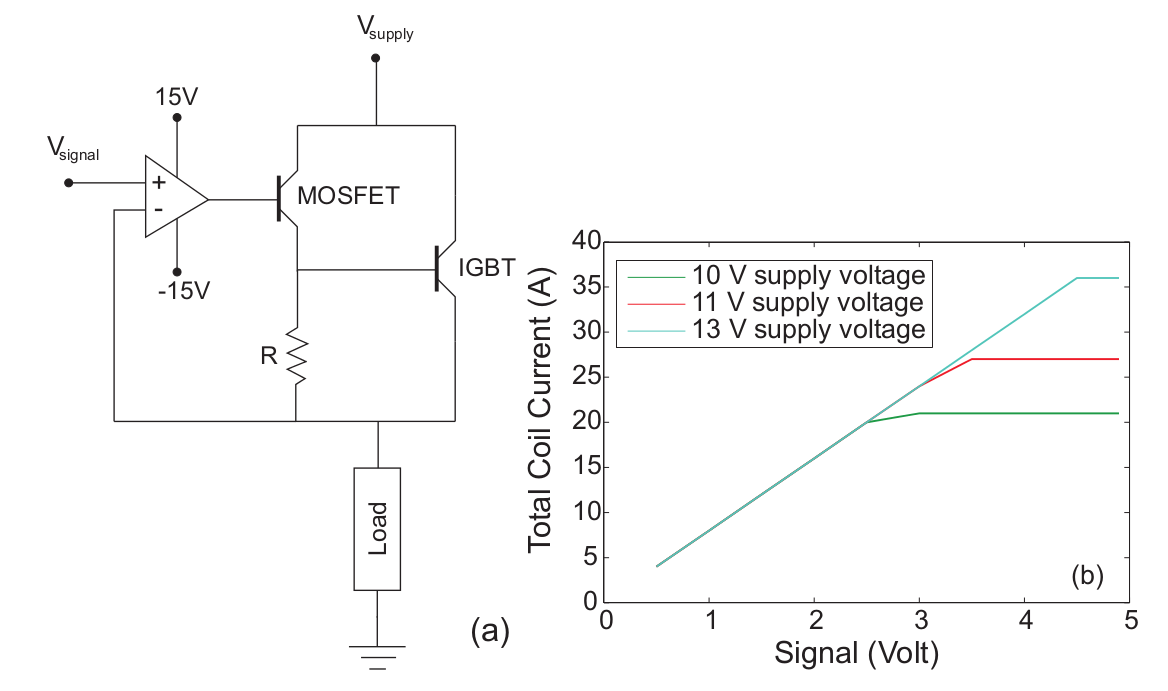
\includegraphics[width=100mm]{current_control.png}
\caption{Current control circuit from \cite{Palittapongarnpim2012}, Fig 3.10, for feedback control the coil current}
\label{fig:pfeedbackcircuit}
\end{figure}

\citet{Dieckmann2001} has a detailed description of an IGBT based switching circuit, with high current, and $\approx 60 \mu \mathrm{s}$ switching time. The complete circuit is shown on Figure \ref{fig:multipath}, and so complex because they are using it to switch multiple coils, for a magnetic trap and Feschbach resonances as well. They use IXYS IXGN200N60A, supported by diodes IXYS DSEI2×101, and preloaded capacitors (200V) to speed things up. They mention computer control of the IGBT currents but no details provided, thus I think it's the same simple method as mentioned earlier (operating in the saturation region) which is supported by the spec sheet of that IGBT model.

\begin{figure}[ht!]
\centering
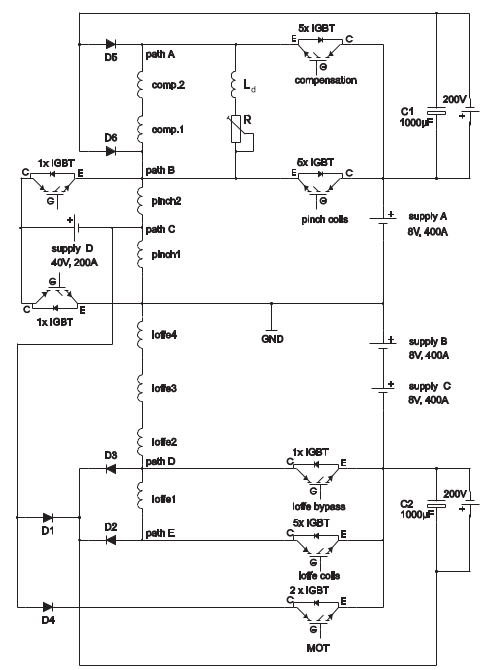
\includegraphics[width=120mm]{multipath_switching.png}
\caption{Current control circuit from \citet{Dieckmann2001}}
\label{fig:multipath}
\end{figure}

There are other papers mentioning IGBT performance as well without circuit diagrams: \citet{Bolpasi2012} has Max 400A current, switch on in $100 \mu \mathrm{s}$, off in $40 \mu \mathrm{s}$. \citet{Schuricke2011} use max 35A, IGBT with part number EUPEC FZ 800 R16 KF4, switching time $400 \mu \mathrm{s}$, trying to minimize Eddy currents by the arrangement of the coils and metal parts, but not totally successful. \citet{Holynski2012} is switching 80-100A with IGBT, they mention that the maximum current drops due to thermal effects (heating of the collector-emitter region,a nd they use oil pumping for cooling. \citet{Pasquini2007} has similar arrangement, but only proposed yet: using the resistance of an IGBT to control the current of coils.

On the other side, \citet{Pant2011} is using sophisticated, versatile, thus maybe too complex MOSFET control circuit, see Figure \ref{fig:mosfet}, but they have only 5A to control.

\begin{figure}[ht!]
\centering
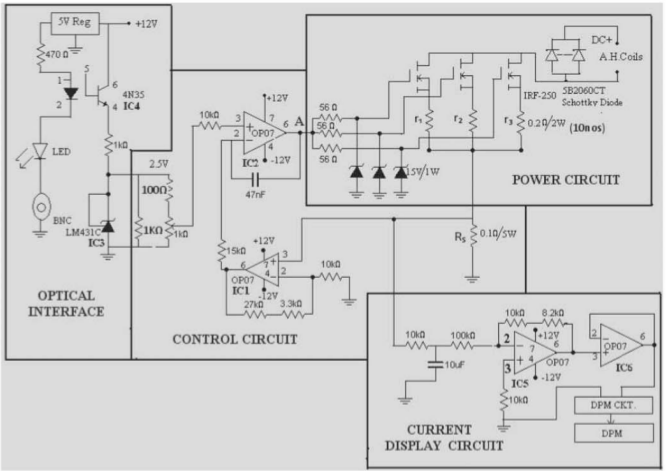
\includegraphics[width=130mm]{mosfetcircuit.png}
\caption{Current control circuit from \citet{Pant2011}}
\label{fig:mosfet}
\end{figure}

Lots of interesting points in \citet{Gorelik2002}, where the whole thesis seem to work on similar problems that are considered here, would warrant further inspection. In general about the circuits, construciton and cooling, maybe some interesting idea or details can be gotten from \citet{Meyrath2004}.

For current measurement, the sense resistors are probably not that good (the one with the NIST notes have too low maximum current), other sensors based on Hall effect, or Giant Magnetic Resonance should be better considered.

\section{Conclusions}

Based on what I've seen the IGBT circuits seem to be working well in a lot of laboratories with similar requirements as here. For teh current generation of devices, their stability, wide spread, industry support for better devices should just make them even better now.

In after assemly, the coil parameters (resistance, inductance) should be measured well, and it should be possible to create a simple enough circuit model (as in \citet{Deissler2003}) to predict the behaviour, since the inductance will have the biggest effect on the overall system behaviour.

Also, the current feedback could be tried in a test circuit on a low current value (so there's no need for water cooling first, and it's less dangerous), though have to be careful about the maximum applied gate volage, it will likely be quite low value, given the output characteristics, like Figure \ref{fig:cm600dy}.

In the overall setup, the trickiest part is the overall resistance budget, given that the theoretical maximum of the power supply is $34 \mathrm{m\Omega}$ (15V/440A, Agilent 6690A).

\section{Appendix: Companies}

\begin{itemize} \itemsep -2pt
\item ABB \url{http://www.abb.com}
\item Dynex \url{http://www.dynexsemi.com}
\item Fuji Electric \url{http://www.fujielectric.com}
\item Infineon \url{http://www.infineon.com}
\item International Rectifier \url{http://www.irf.com}
\item IXYS \url{http://www.ixys.com}
\item Microsemi \url{http://www.microsemi.com}
\item Nihon Inter Electronics Corp \url{http://www.niec.co.jp}
\item Powerex \url{http://www.pwrx.com}
\item Vishay \url{http://www.vishay.com}
\end{itemize}

\bibliographystyle{unsrtnat}
\bibliography{quadcoil}

\end{document}